\documentclass[a4paper,12pt,oneside,openright]{book}
\usepackage[utf8x]{inputenc}
 
\usepackage{bookman}
\usepackage{graphicx}

\usepackage{subfig}
\usepackage{listings}
\usepackage{fancyhdr} 
\usepackage{color}
\usepackage[table]{xcolor}
\usepackage[T1]{fontenc}
\usepackage{float}
\usepackage{ifthen}
\usepackage{geometry}
\geometry{a4paper, portrait, margin=1in}
\usepackage{afterpage}
\usepackage{multirow}
\usepackage{multicol}
\usepackage{rotating}
\usepackage{tikz}
\usepackage{hyperref}
\usepackage{inconsolata}
\usepackage{url}
\usepackage{textgreek}
\usepackage{ragged2e}
\usepackage{inputenc}
\usepackage{babel}
\usepackage{hyperref}
\usepackage{amssymb}
\usepackage{pifont}
\usepackage[titles]{tocloft}
\usepackage{wrapfig}
\usepackage{floatrow}
\usepackage{csquotes}
\cftsetindents{figure}{0em}{3em}
\cftsetindents{table}{0em}{3em}

\usepackage{url}
\def\UrlBreaks{\do\/\do-}
\usepackage{breakurl}

\usepackage{etoolbox, tocloft}
\preto\figure{%
  \ifnum\value{figure}=0\addtocontents{lof}{{\bfseries Chapter \thechapter\vskip5pt}}\fi
}


\definecolor{mygreen}{rgb}{0,0.6,0}
\definecolor{mygray}{rgb}{0.5,0.5,0.5}
\definecolor{mymauve}{rgb}{0.58,0,0.82}

\newtheorem{theorem}{Theorem}

\lstset{ %
  backgroundcolor=\color{white},   % choose the background color
  basicstyle=\footnotesize,        % size of fonts used for the code
  breaklines=true,                 % automatic line breaking only at whitespace
  captionpos=b,                    % sets the caption-position to bottom
  commentstyle=\color{mygreen},    % comment style
  escapeinside={\%*}{*)},          % if you want to add LaTeX within your code
  keywordstyle=\color{blue},       % keyword style
  stringstyle=\color{mymauve},     % string literal style
}

\pagestyle{fancy}
\fancyhead[RO]{\footnotesize{\thepage}}
\fancyhead[LO]{\footnotesize{\rightmark}}
\fancyfoot{}

\tolerance=1
\emergencystretch=\maxdimen
\hyphenpenalty=10000
\hbadness=10000

\newcommand{\cmark}{\ding{51}}%
\newcommand{\xmark}{\ding{55}}%
\renewcommand{\footnotesize}{\scriptsize}
 
\begin{document}
\newgeometry{centering}
\begin{titlepage}
    \begin{center}
        \begin{minipage}{0.25\textwidth}
                \scalebox{0.3}{
\includegraphics{figures/DCTI Logo - Simplu.png}}
        \end{minipage}
        \begin{minipage}{0.35\textwidth}
            \begin{flushleft}
                \scalebox{0.3}{
\includegraphics{figures/logo-ac.png}}
            \end{flushleft}
        \end{minipage}
        \begin{minipage}{0.3\textwidth}
            \begin{flushright}
                \scalebox{0.3}{
\includegraphics{figures/UPTlogo.JPG}}
            \end{flushright}
        \end{minipage}
    \end{center}
    
    \noindent\rule{\textwidth}{1pt}\\[4.8cm]
    
    \begin{center}
        { \Huge \bfseries \textsc {DC - Benchmarking} }\\[1cm]
        { \large \bfseries Project realised by \textit{The Happy Group}\\[3.0cm]
        \begin{flushright}
            \large
            Students:\\[0.15cm]\textbf{Nicolae Bunea}\\
            \textbf{Sebastian Boghiu}\\
            \textbf{Andrei Dragan}\\
            \textbf{Darius Dobra}\\
            \textbf{Eusebiu Florea}\\[3cm]
        \end{flushright}
        {\small Timișoara \\April, 2025}
    \end{center}
\end{titlepage}
\restoregeometry
\shipout\null

\setcounter{page}{1}
%\tableofcontents

\chapter{Read Me}

You can remove this file (and this chapter) after you finish working on the documentation. Consider it as a cheat sheet for your (probably first) documentation and also as a guideline for using \LaTeX{} and Overleaf. I am sure you will use \LaTeX{} even for other occasions (like writing a CV more professionally, writing your diploma project, writing an article, for a poster, and so on). Besides this file, the others can be kept because I expect you to follow the guidelines and the structure I have created for you. You just have to fill in the information under some sections and answer to a couple of questions.

\noindent
{\color{red} \rule{\linewidth}{0.5mm} }
The most important thing I am expecting from you while writing this documentation is to learn and make an idea of how such a tool works. You will not receive a lower mark if the documentation doesn't look the best, but I expect you to \textbf{use Overleaf}. 

\noindent
{\color{red} \rule{\linewidth}{0.5mm} }

Remember: 
\begin{itemize}
    \item In order to save your changes, you have to recompile the project from the 'Recompile' green button.
    
    \item A disadvantage of using Overleaf (free edition) in big teams is that the owner of the project can share the project with only one editor, so the other teammates won't be able to make changes to the files. But you can split your documentation into tasks and you can combine your work in the end.
    
    \item Each one of you will have to upload the documentation on Campus. I will read only one documentation from each team (they have to be the same) and I will read only the answers to the \textbf{conclusions} chapter (I expect them to be unique because I assume each one of you has a different opinion).
    
    \item Your documentation should not be longer than 12 pages. I know for some of you it's harder to come up with a lot of words, but remember that the documentation also has \textbf{tables}, \textbf{code sequences}, \textbf{figures}.
    
\end{itemize}

\section{How to insert code?}

Did you know you can list code in \LaTeX{}? You just have to copy-paste it from the IDE inside a \textbf{lstlisting} element. You can provide a caption which explains that sequence of code. The caption doesn't have to be long, but please make it explanatory enough. Please do not copy the entire code, but we'll discuss about this later.

I've attached a short snip of code from one of my previous projects. You can see that the caption is pretty clear and it is longer than just a couple of words, which is good for the reader, who has to understand not only what the code does, but \textbf{\textit{why}} you have included a specific code sequence. 

\begin{lstlisting}[caption={Checking if the user has selected the role in the application checking a radioButton according to his role (doctor or patient). If any radioButton has been selected, the register button changes is colour and becomes enabled.}, language=Java]
    
    radioGroup = findViewById(R.id.rol);
    registerButton = findViewById(R.id.registerButton);
    radioGroup.setOnCheckedChangeListener((group, checkedId) -> {
        RadioButton checkedRadioButton = radioGroup.findViewById(checkedId);
        boolean isChecked = checkedRadioButton.isChecked();
        if(!isChecked){
            setRegisterButtonStyle(false, "#ffe082");
        } else {
            setRegisterButtonStyle(true, "#ffb300");
        }
    });
\end{lstlisting}

Also, we can choose to add a list of all code sequences, a list of all tables, and also a list with all figures, but this kind of lists are recommended for more elaborate documents. I remember the fact that \textbf{you shouldn't write a document with more than 12 pages}. 

\section{How to insert equations?}

You can also list equations (probably the score's formula, right?).

\begin{equation}
z = (x - u)/s
\end{equation}

\section{How to insert tables?}

\begin{table}[ht]
\centering
\begin{tabular}{|l|l|l|l|l|l|l|l|}
\hline
\textbf{Nr} & \textbf{CPU}  & \textbf{Cores} & \textbf{Clock} & \textbf{RAM} & \textbf{OS} & \textbf{...} & \textbf{Score} \\ \hline
1           & Core i5 7600K & 4/4            & 3.50           & 4096         & Win10 Home  & ...          & 1205           \\ \hline
2           & Ryzen 7 1700X & 8/16           & 3.00           & 8192         & Win8.1 Pro  & ...          & 1622           \\ \hline
\end{tabular}
\caption{Your caption describing the table.}
\label{example-table}
\end{table}

You definitely don't have to worry about learning or understanding details about how tables work in Overleaf, the syntax used to generate a table, and other things. Just use a generator (I suggest you to use \cite{table-generator}) and your job will be a lot easier. The table \ref{example-table} is pretty good.

\section{How to insert images?}

You can set a lot of parameters for the pictures you choose to insert in the documentation. You can find out more about them here \cite{image-documentation}. For figure \ref{statistics-diagram} I chose the width and also I wanted to keep the aspect ratio unchanged. Inside the folder called \textbf{figures} you can store the figures you want to use. Don't delete the ones that are there now because they are used on the first page.

\begin{figure}[H]
    \centering
    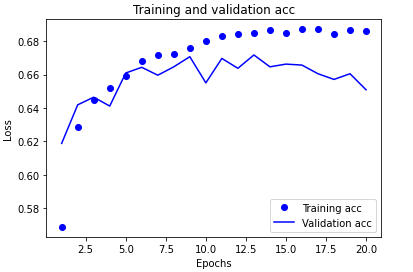
\includegraphics[width=11cm,keepaspectratio]{figures/training.png}
    \caption{Monitoring the training and validation accuracy. In this figure we can see that the model starts overfitting at around the 10th epoch.}
    \label{statistics-diagram}
\end{figure}
\chapter{Introduction}

HappyMark is a benchmarking tool written in Java code that test the CPU and the memory .

\section{Context}

\begin{itemize}
  \item We have made an application that tests the CPU's reading, computation, and writing speed by running a loop.
  \item The app also tests how fast the communication between the CPU and RAM is.
  \item We are also testing storage memory by testing how fast we can read and write from files.
  
\end{itemize}

\section{Motivation}

\begin{itemize}
  \item One would choose our app because it is easy to use, it clearly displays how much time it takes to run the test, and compares your result with the average result.
  
  \item This tool was inspired by Cinebench and UserBenchmark. We like how UserBenchmark displays its results and decided to do something similar. We run the test and then compare the time it took to finish with a reference.

\end{itemize}

\chapter{State of the art}

\section{Cinebench}

\begin{itemize}
  \item Cinebench is a free benchmarking tool developed by Maxon, designed to evaluate your computer's CPU and GPU performance by rendering complex 3D scenes. It simulates real-world tasks to assess how well your hardware handles intensive workloads, making it useful for anybody stress-testing their desktop.
  \item Cinebench provides separate tests for single-core and multi-core CPU performance, as well as GPU rendering capabilities, offering a comprehensive view of your system's processing power. It's widely used by hardware reviewers, system builders, and enthusiasts to compare performance across different systems and configurations.
\end{itemize}

\section{UserBenchmark}

\begin{itemize}
  \item UserBenchmark is a free benchmarking tool and website that allows users to evaluate and compare the performance of their computer hardware, including CPUs, GPUs, SSDs, HDDs, RAM, and USB drives.
  \item UserBenchmark displays the results in percentages. For example, if a CPU has scored 120\% in the test, that means it completed the test 20\% "average" CPU.
  \item It should be noted that the CPU test in UserBenchmark faced some backlash for placing too much importance in single-core performance.
\end{itemize}

\section{Comparison}
\begin{table}[ht]
\centering
\begin{tabular}{|l|l|l|l|}
\hline
                      & \textbf{Cinebench}  & \textbf{UserBenchmark} & \textbf{HappyBench}  \\ \hline
Single-core only test & Yes                 & No                     & No                      \\ \hline
Hardware Tested       & CPU, GPU            & CPU, GPU, RAM, SSD, USB& CPU, SSD             \\ \hline
Results format        & Score               & Percentage             & Time, Percentage \\
\hline
\end{tabular}
\label{example-table}
\end{table}



\chapter{Design and implementation} 

\begin{itemize}
  \item  First of all, we followed the template offered by the project sheets. We used Java as a programming language and IntelliJ as IDE. We created functionalities for the bench, logging and the timing, whom are the base of a benchmark. Offers the measure in time(nanoseconds), and we used the package approach for each piece that we needed in order to knock down the benchmark in a organised way.
  
  \item \textbf{Briefly} describe the used algorithms and other \textbf{special features}. Do not add source code (entire files), \textbf{only} short snippets \textbf{if you feel they are relevant}, and if you want to emphasize anything. In order to test the functionality, we created a "Dummy Benchmark" in order to test the overall functionality:
  \begin{itemize}
      \item Dummy: complete a array of N elements with random values
      \item Demo: take N random integers between 0 - 1000 and perform bubble sort
      \item CPU: perform the addition of all prime numbers upon a upper limit
      \item Sleep: the same as CPU but with a different run condition, with a "sleep" time added.
  \end{itemize}

  \item https://github.com/ThorSPB/DC-Project.git
\end{itemize}
\chapter{Usage}

\begin{itemize}
  \item Here, you should include a step-by-step description of how a user should use your benchmark. You should include pictures and screenshots. If you have a UI (which is a \textbf{bonus}), please explain the role of all visible UI elements.
  
  \item Describe the manner your benchmark outputs results (scoring). Is it a graphical representation, a number, or a text file with raw data? The easier and more compact your benchmark score is, the better (e.g. points, running time).
  
  \item Remember that your application has to be: 
    \begin{itemize}
    \item Standalone and portable (Windows 8+ OS mandatory, other OS optional)
    \item Run-able by anyone with a simple click (or double click, command line)
    \item Should not require special input
    \item Should produce output (graphical, text, etc.) that is measurable/comparable against other results on other machines)
    \end{itemize}
\end{itemize}




\chapter{Results}

This chapter is again very important in what means \textbf{analysing}. If in chapter 2, the focus is on comparing methods, here, the focus is on comparing and on interpreting results.

\begin{itemize}
  \item Graphical or numerical representation of the benchmark results using your proposed scores. Highlight what is relevant, do not simply put huge amounts of numbers on paper with no immediate conclusion. 
  
  \item Interesting results: did you capture a specific feature of the hardware you are testing? Did you find anything you were not expecting? Two figures in total for this section should be enough, no need for more.
  
  NOTE: you must gather scores (results) from at least 5 different machines (with different hardware components!). If you run the study on more than 10 machines you will receive a \textbf{bonus}. 
  
  \item Make sure you gather system information for every benchmark result as well (i.e. not just scores, but also hardware configuration, OS, etc.)
  
  \item As an annex to the documentation, you must provide the gathered benchmark scores in tabular form, with enough detail to prove that each score comes from a unique environment.
\end{itemize}







\chapter{Conclusions}

Please also focus on this chapter! I know that sometimes while writing a document, conclusions are the last thing to write, but remember that they are also the last thing to read and might change the reader's overall perspective of the document. I would want you to answer to the following questions and, why not, even some added by yourself. 

\begin{itemize}
  \item \textbf{What did we learn?}
  
  (e.g.) During this semester, we learned X and Y. 
  
  \item \textbf{What mark would I give to me? How much did I contribute to the teamwork (project, application, presentation)? What mark do I think my colleagues deserve?}
  
  (e.g.) If it were up to me, I would give myself \textbf{...}, because even if the project is pretty good, I did (not) help as much as my colleagues. (e.g.) I consider 20\% of the final project is because of me. Also, I want to add that we did (not) indeed work as a team and I think all of us should get the same mark. (or not) 
  
  \textit{Remember each one of you will have to upload the documentation on Campus, but the answers to these questions have to be unique. (this one in particular).}

  \item \textbf{What was hard, what did we enjoy, what did we hate, what did we like and dislike about the CO project?}
  
  \item \textbf{How would you change (improve) the project meetings for the next generation of students?}
  
  I will definitely take into consideration your feedback and I will consider applying your suggestions as I did with most of the ideas gained last year.
  
\end{itemize}

\bibliographystyle{unsrt}
\bibliography{bibliography.bib}

\end{document}